\textbf{Name:} Patrick Harvey\\

\medskip

\textbf{Conspirators:} Chris O'Neil\\

\medskip

\textbf{Self-Referential Linkage:}\\
\url{https://www.overleaf.com/read/jwptqkrxjbkr}\\
\url{https://github.com/P-Harvey/csys303_assignments}\\

\medskip
\medskip

\hrule

\medskip


\begin{enumerate}

\item (3 + 3)
  Reproduce Bohn and Magnasco's Figs. 2a and 2b in~\url{https://arxiv.org/pdf/cond-mat/0607819}:

  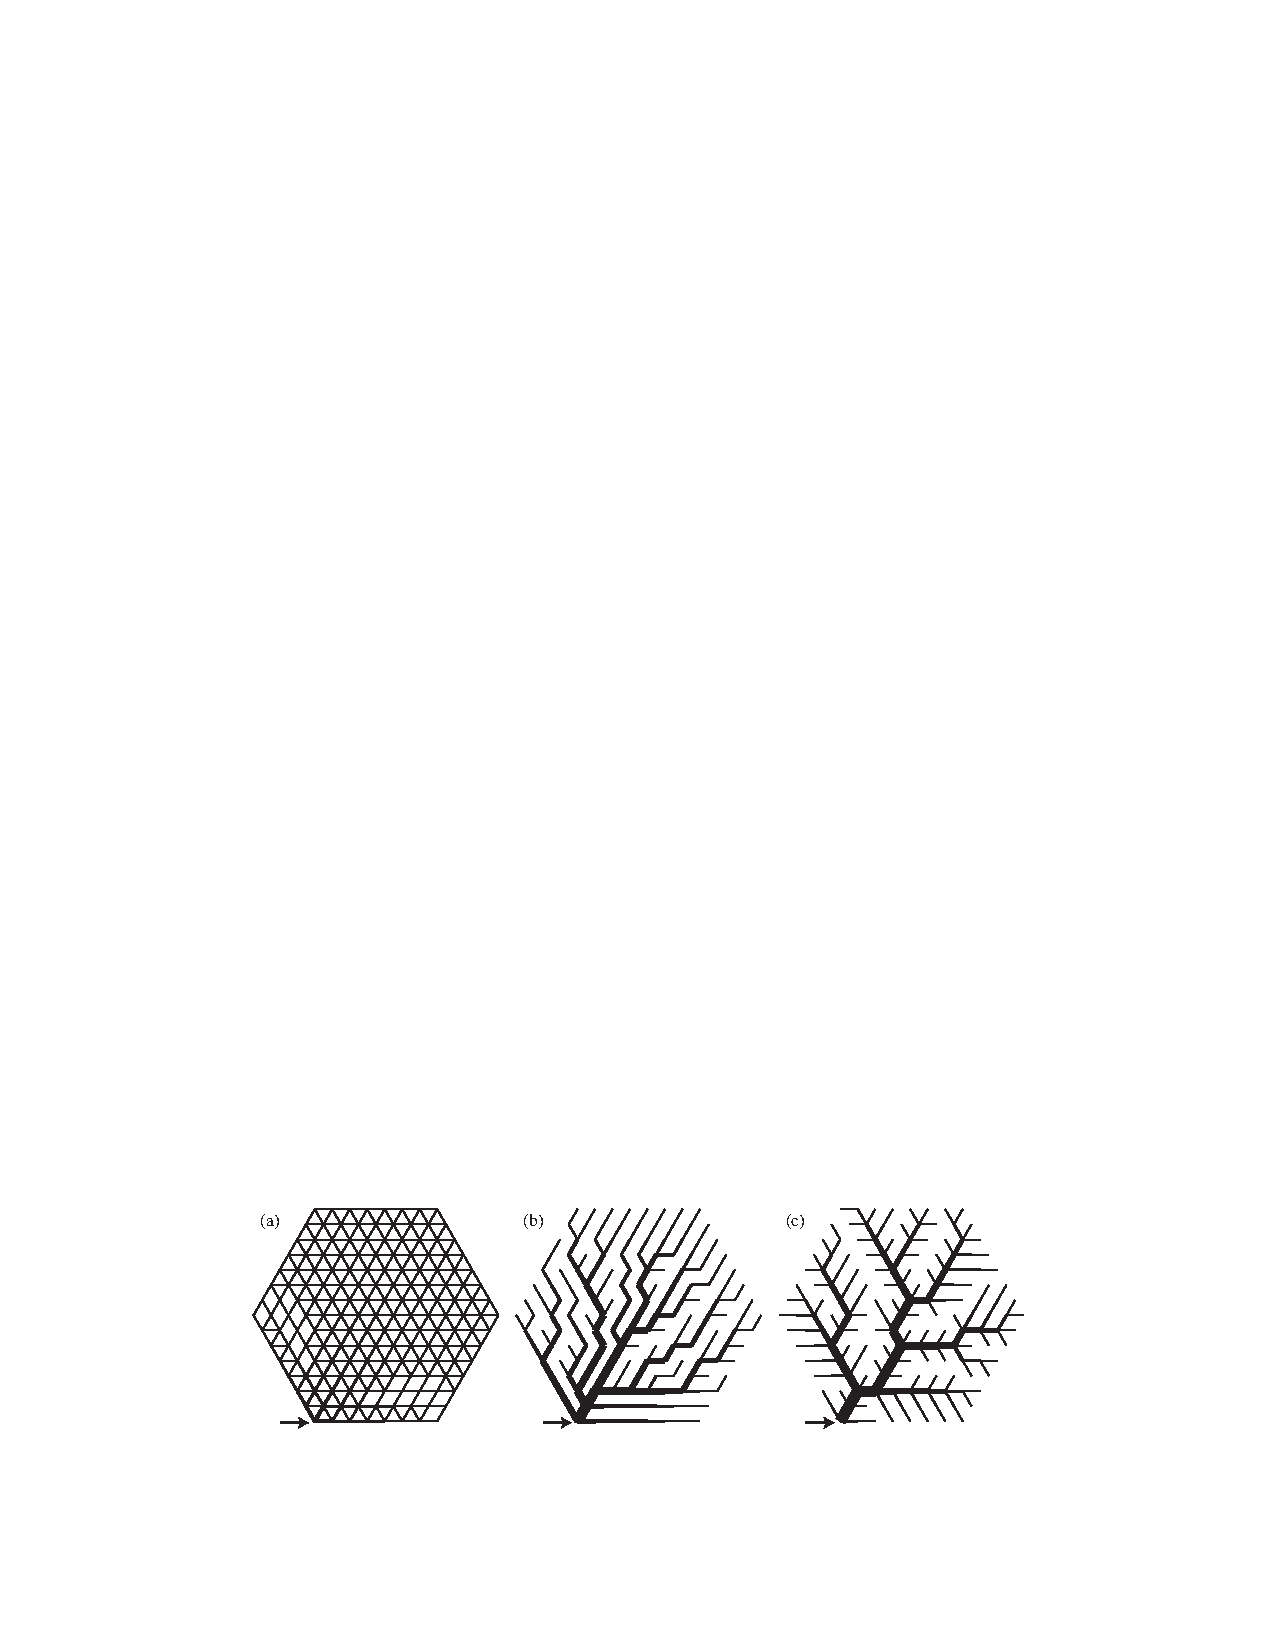
\includegraphics[width=\textwidth]{bohn2007a_fig2.pdf}

  Steps are given below but please read through the paper to understand how they set things up.

  The full team is encouraged to work together on Teams.

  %% I check the paper again and that constraint on conductances can be viewed as a constraint on building material for the network.  Everything derives from a Lagrange multiplier set up and has parallels with the HOT model, size-area density, and the (erroneous) West et al. work for blood networks.

  \begin{enumerate}
  \item Done (previous assignment):    
    Construct an adjacency matrix $\m{A}$ representing the hexagonal lattice
    used in~\cite{bohn2007a}.  Plot this adjacency matrix.
  \item (3 + 3)
    Run a minimization procedure to construct Figs. 2a and 2b which
    correspond to $\gamma=2$ and $\gamma=1/2$.
    Steps:
    \begin{enumerate}
    \item 
      Set each link's length to 1 (the $d_{kl}$).
      The goal then reduces to minimizing the cost
      $$
      C 
      = 
      \sum_{k,l} 
      \left| 
      I_{kl}
      \right|^{\Gamma}
      $$
      where $I_{kl}$ is the current on link $kl$
      and $\Gamma = 2\gamma/(\gamma+1)$.
    \item
      Place
      a current source of nominal size $i_0$ at one node
      (as indicated in Fig.~2 above).
    \item 
      All other nodes are sinks, drawing a current of 
      $$
      i_{k} = 
      - \frac{i_{0}}
      {N_{\textnormal{nodes} - 1}}.
      $$
    \item 
      Suggest setting $i_0 = 1000$ (arbitrary but useful value given the size of the
      network).
    \item 
      Generate an initial set of random conductances for each link,
      the $\{\kappa_{kl}\}$.
      From the paper, these must sum to some global constraint as
      $$
      K
      =
      \left(
      \sum_{k,l}
      \kappa_{kl}^{\gamma}
      \right)^{1/\gamma}.
      $$
      This constraint is meant to represent a limitation on the amount of material
      that can be used to build the network.

      Note: There seems to be no reason not to set $K = 1$.
      However, taking the initial value of $K$ determined by
      the initial set of random conductances would work.

      To our notational peril, we now have a lot of $k$ types on deck.
    \item 
      Solve the following to determine the potential $U$ at each node,
      and hence the current on each link using:
      $$
      i_{k}
      =
      \sum_{l}
      \kappa_{kl}(U_{k}-U_{l}),
      $$
      and then
      $$
      I_{kl} = \kappa_{kl}(U_{l} - U_{k}).
      $$
      Note: the paper erroneously has $I_{kl} = R_{kl}(U_{l} - U_{k})$ below
      equation 4; there are a few other instances of similar
      miswritings of $R_{kl}$ instead of $\kappa_{kl}$.
    \item 
      Now, use scaling in equation (10) to compute a new set of $\{\kappa_{kl}\}$
      from the $I_{kl}$.  Everything boils down to 
      $$
      \kappa_{kl} \propto | I_{kl} |^{-(\Gamma-2)},
      $$
      where the constant of proportionality is determined
      by again making sure 
      $
      K^{\gamma}
      =
      \sum_{k,l}
      \kappa_{kl}^{\gamma}.
      $
    \end{enumerate}

    %% Antioch joke
    %%  Bonus: Please see reference 1 in~\cite{bohn2007a} for a random
    %%  connection to the next assignment's code name.

    Some help---Let's sort out the key equation:
    $$
    i_{k}
    =
    \sum_{l}
    \kappa_{kl}(U_{k}-U_{l}).
    $$
    Each time we loop around through
    this equation, we know the $i_{k}$ and the $\kappa_{kl}$
    and must determine the $U_{k}$.  
    In matrixology, we love $\Axb$ problems so let's see
    if we can fashion one:
    $$
    i_{k}
    =
    \sum_{l}
    \kappa_{kl}(U_{k}-U_{l})
    $$
    $$
    =
    \sum_{l}
    \kappa_{kl} U_{k}
    -
    \sum_{l}
    \kappa_{kl} U_{l}
    $$
    $$
    =
    U_{k}
    \sum_{l}
    \kappa_{kl}
    -
    \sum_{l}
    %%    [\m{K}^{\textnormal{T}}]_{kl} U_{l}
    \m{K}_{kl} U_{l}
    $$
    $$
    =
    \lambda_{k}
    U_{k}
    -
    [
      %%    \m{K}^{\textnormal{T}} \vec{U}
      \m{K} \vec{U}
    ]_k
    $$
    where we have 
    set 
    $
    \lambda_{k}
    =
    \sum_{l}
    \kappa_{kl},
    $
    the sum of the $k$th row of the matrix $\m{K}$.
    We now construct a diagonal matrix $\Lambda$ with
    the $\lambda_{k}$ on the diagonal, and obtain:
    $$
    \vec{i}
    =
    \left(
    \Lambda
    -
    %%    \m{K}^{\textnormal{T}} 
    \m{K}
    \right)
    \vec{U}.
    $$
    The above is in the form $\Axb$ so we can
    solve for $\vec{U}$ using standard features
    of R, Matlab, Python, \ldots\ (hopefully).

    
   \solutionstart

   Given our desired end-state ($\textnormal{argmin}{\left(C\right)}$) where:
   
   $$
   C 
   = 
   \sum_{k,l} 
   \left| 
   I_{kl}
   \right|^{\Gamma}
   $$
   
   With $I_{kl}$ being the current on link $kl$ and $\Gamma = 2\gamma/(\gamma+1)$.
   We can approach this problem in a variety, or combination, of ways.\\

   It took me a minute (or maybe a quarter of an hour, in minutes$_{A000217}$),
   but I look at this as an application of spectral graph theory.
   We will begin with the association of matrices to a graph.
   Specifically, we will use the adjacency and the Laplacian matrices.\\

   First a detour. The integer sequence ($A000217$) referenced above is defined as:

   \begin{equation}
        a(n) = \binom{n+1}{2}
   \end{equation}

   This gives the integer series of triangular numbers (or generalized $k$-gonal numbers).
   We are interested in $a(n=8)=36$ for a few reasons.
   First, this is the \cdots
   
   % The general theme is then, first, to compute or estimate the eigenvalues of such matrices, and, second, to relate the eigenvalues to the structural properties of the graph. 

   % I will pursue a method of solving this problem using properties of geometric shapes on manifolds, Hipparchus-Schroeder-Tamari-Stasheff (HSTF) associahedrons, and analytic chord diagrams.

   % Let's start with a proposition for partitioning a convex polygon with $(n+1)$ edges ($n+1=6$, or better yet, $2(n+1)=2 \cdot 3$).

   % Proposition: We can view each vertex of this lattice as a chord diagram.

    % We know that our lattice is a combination of three possible isometries defined by:
   
   % \begin{align*}
   %     S_{ij} &=
   %     \begin{bmatrix}
   %          1  &  0  &  0  &|&  1 \\
   %          0  & -1  &  0  &|&  0 \\
   %          0  &  0  & -1  &|&  0
   %     \end{bmatrix}\\
   %     S_{jk} &=
   %     \begin{bmatrix}
   %          -1 &  0  &  0  &|&  0 \\
   %          0  &  1  &  0  &|&  1 \\
   %          0  &  0  & -1  &|&  0
   %     \end{bmatrix}\\
   %     S_{ik} &=
   %     \begin{bmatrix}
   %          -1 &  0  &  0  &|&  0 \\
   %          0  &  -1 &  0  &|&  0 \\
   %          0  &  0  & 1   &|&  1
   %     \end{bmatrix}
   % \end{align*}
   
   % BREAK
   
   % \begin{equation}
   %     U = 
   %     - \frac{
   %     \sum_{ijk} {S_{ij}S_{jk}S_{ki}}
   %     }
   %     {
   %     \left| {\sum_{ijk} {S_{ij}S_{jk}S_{ki}} } \right|
   %     }
   % \end{equation}

   % Where $S_{i} = \pm 1$ for the presence or absence of link...
   \clearpage

   The following \href{https://github.com/P-Harvey/csys303_assignments/blob/218b0b95c67ab3bb6decab0bb0a05d5ac9a6500a/plharvey_18/Flat_Lattice.ipynb}{
   Notebook} has several iterations of plot generation. A few are included below:

   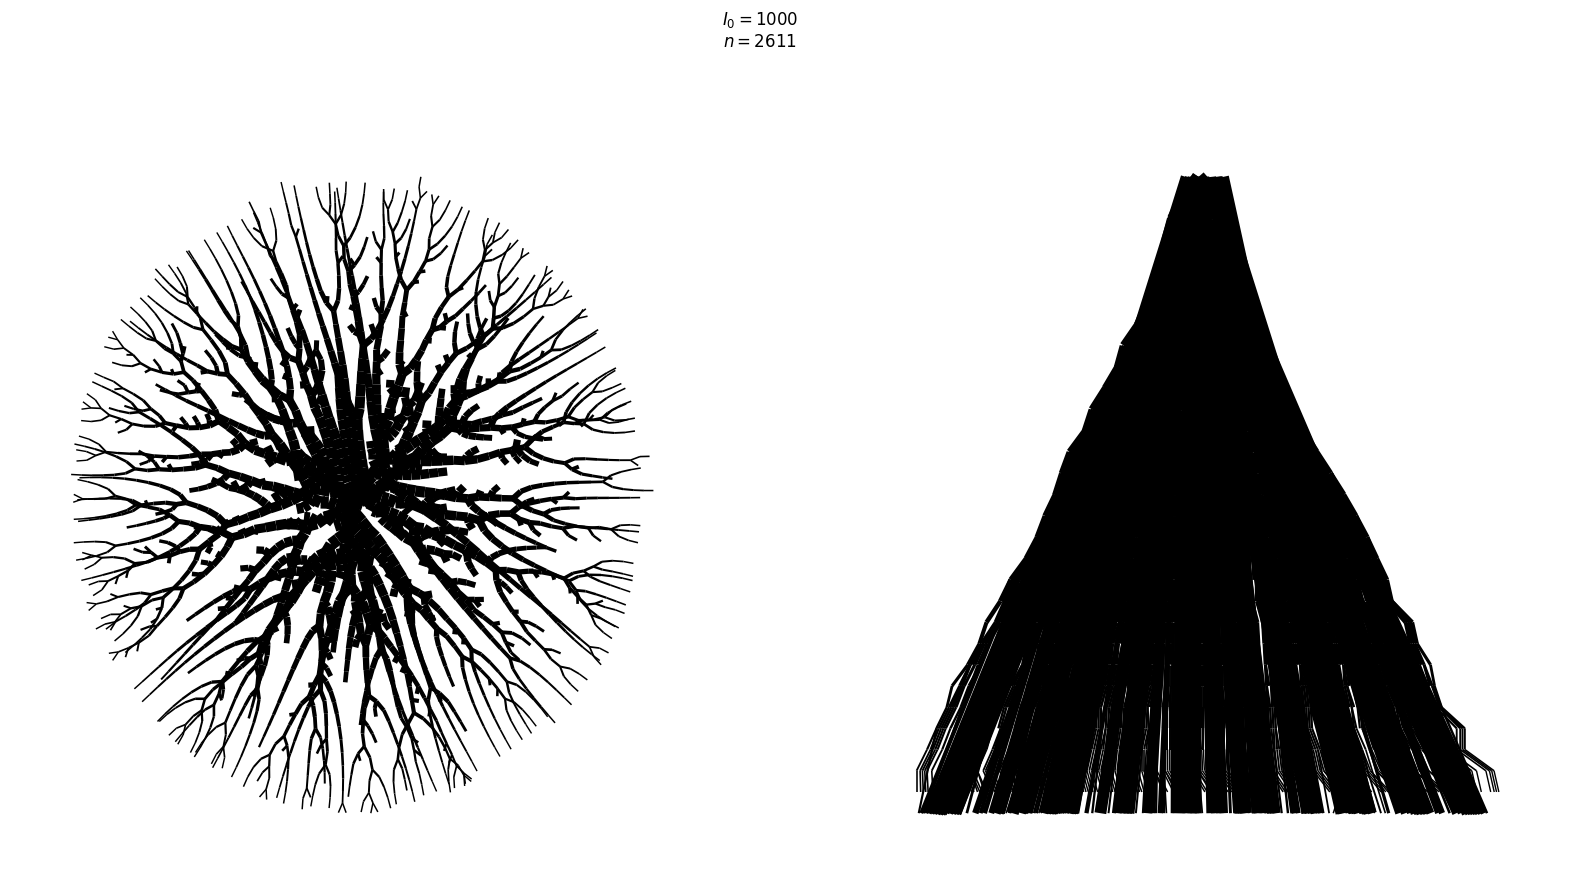
\includegraphics[width=\textwidth]{figures/bigg_lats.png}\\
   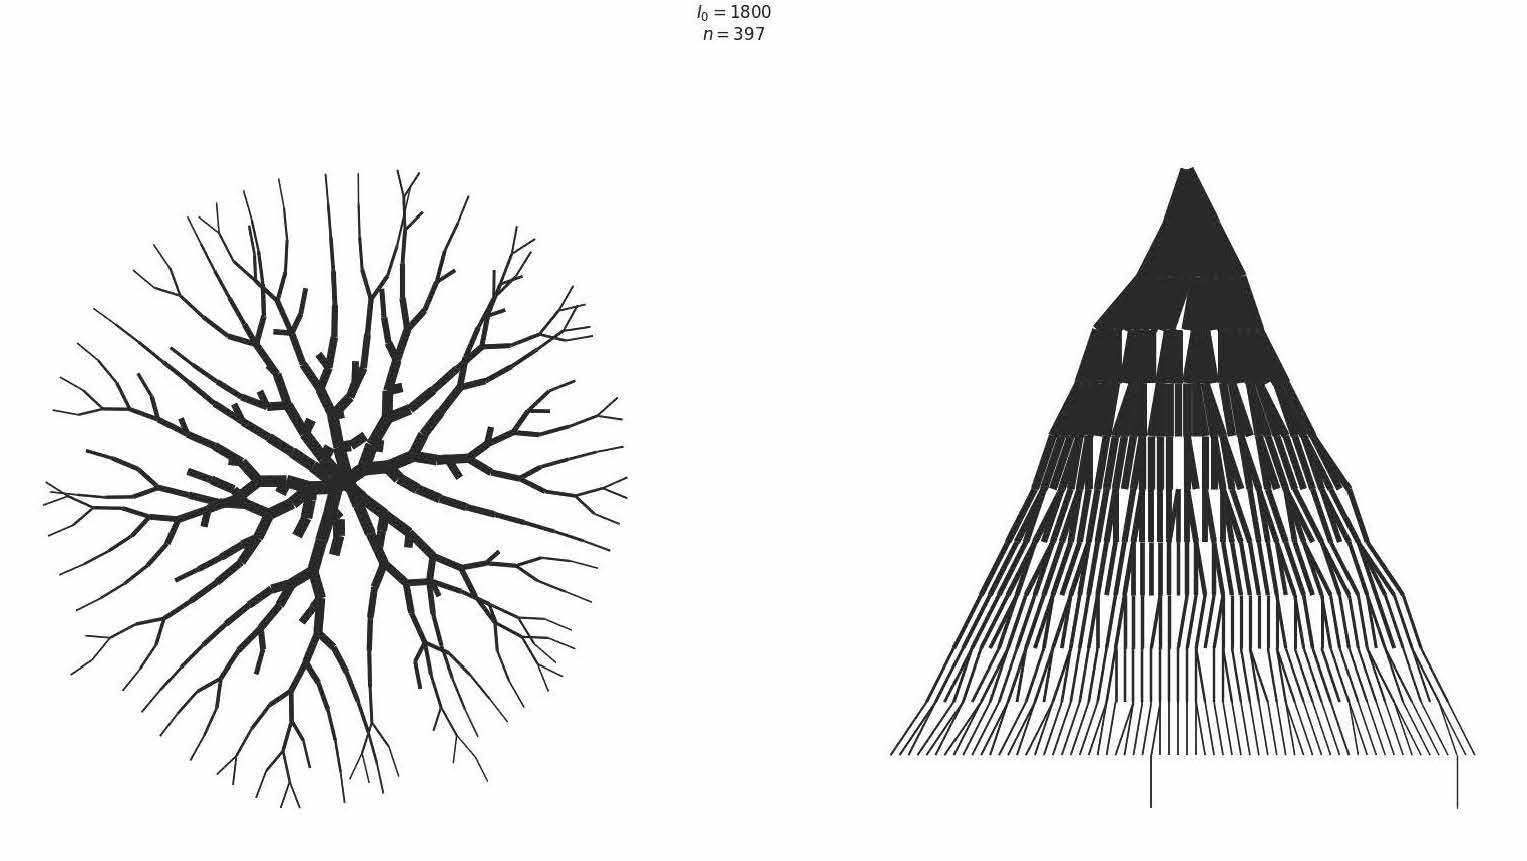
\includegraphics[width=\textwidth]{figures/I_0_1800_n12_397.jpg}\\
   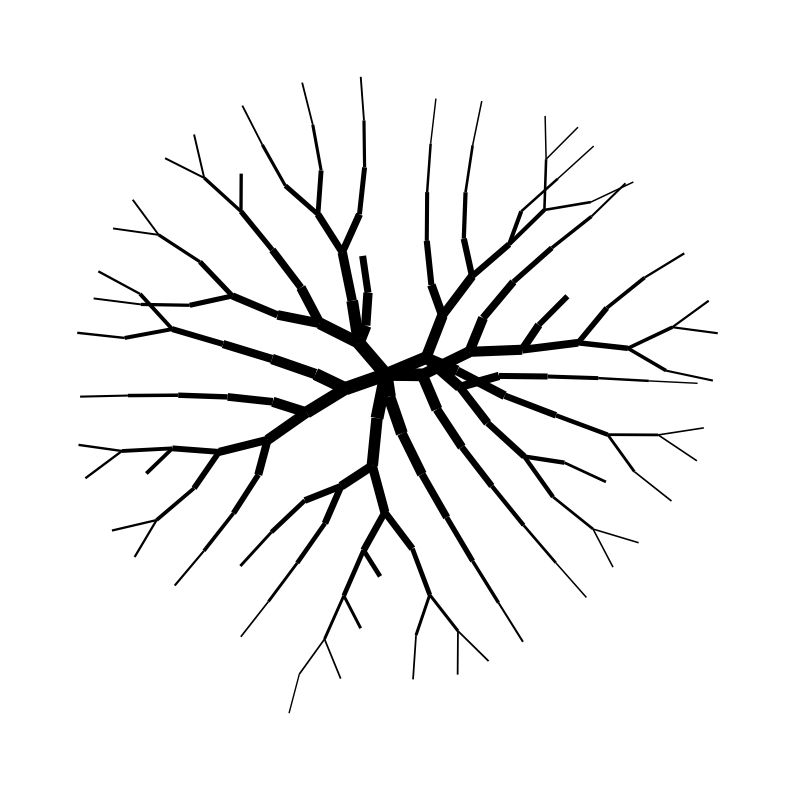
\includegraphics[width=\textwidth]{figures/lattice_1.png}\\
   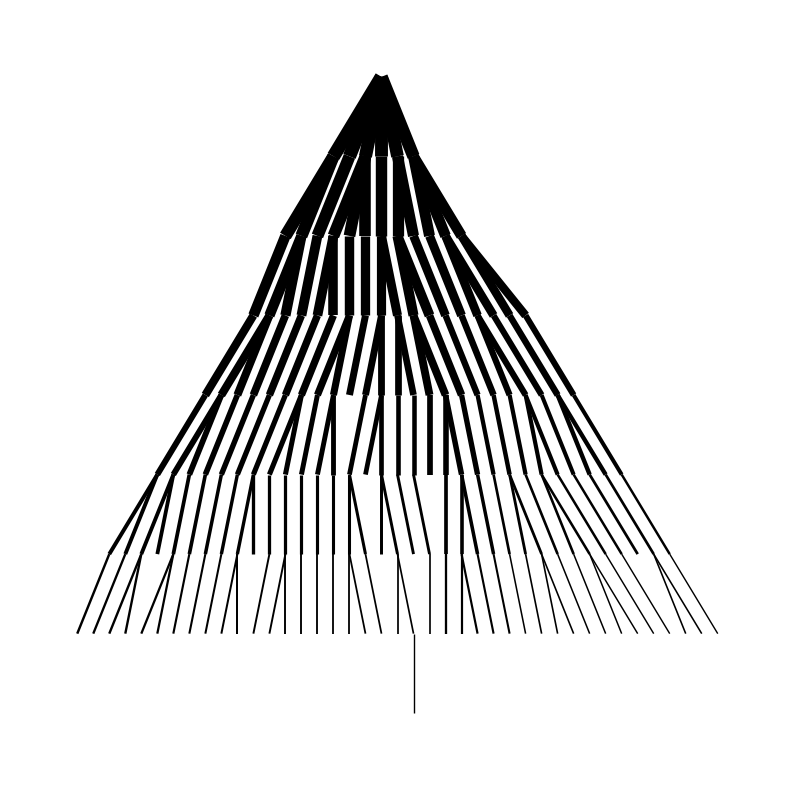
\includegraphics[width=\textwidth]{figures/lattice_2.png}
   \clearpage
   
   \includegraphics[width=\textwidth]{figures/lattice_n_100.png}\\
   Wanted to get this lattice energized, but not enough time in the day.

   \solutionend


    

    
  \end{enumerate}

  %%%%%%%%%%%%%%%%%%%%%
  %% once assignment 04
  %%%%%%%%%%%%%%%%%%%%%


\end{enumerate}


